%! TeX program = lualatex
\documentclass[12pt,a4paper]{article}

\usepackage[nil]{babel}
\usepackage{unicode-math}
\usepackage[svgnames]{xcolor}
\usepackage{lmodern}
\usepackage{graphicx}
\usepackage{wrapfig}
\usepackage{float}
\usepackage{parskip}
\usepackage[font=small,labelfont=bf]{caption}
\usepackage{hyperref}

\babelprovide[import=el, main, onchar=ids fonts]{greek} % can also do import=el-polyton
\babelprovide[import, onchar=ids fonts]{english}

\babelfont{rm}
          [Language=Default]{Liberation Sans}
\babelfont[english]{rm}
          [Language=Default]{Liberation Sans}
\babelfont{sf}
          [Language=Default]{Liberation Sans}
\babelfont{tt}
          [Language=Default]{Liberation Sans}
\hypersetup{
	colorlinks=true,
	linkcolor=blue,
	filecolor=blue,      
	urlcolor=blue,
	pdftitle={An Example},
	pdfpagemode=FullScreen,
}

\urlstyle{same}

%Enter Title Here
 \title{Project-plan v0.1 \\ LibShare}
\author{\textbf{Ονόματα / ΑΜ / Έτος:} \\ Γρηγόρης Καπαδούκας / 1072484 / 4\textdegree \\ Χρήστος Μπεστητζάνος / 1072615 / 4\textdegree \\ Νικόλαος Αυγέρης / 1067508 / 5\textdegree \\ Περικλής Κοροντζής / 1072563 / 4\textdegree}

\begin{document}

\makeatletter
\begin{center}
	\LARGE{\@title} \\
	\pagebreak
\end{center}
\begin{LARGE}\@author\end{LARGE} \\
\pagebreak

%Insert Body Here
\section{Χρονοπρογραμματισμός Έργου}
Εφόσον σύμφωνα με την εκφώνηση υποθέτουμε ότι έχουμε μόλις αποφοιτήσει και σκοπεύουμε να υλοποιήσουμε το έργο που προτείνουμε πραγματικά, ο παρακάτω χρονοπρογραμματισμός υποθέτει ότι σκοπεύουμε στη δημιουργία μιας startup εταιρίας.

Άρα με σκοπό τον χρονοπρογραμματισμό του έργου που θα υλοποιούσαμε έχουμε χωρίσει το project σε επιμέρους tasks. Έχουμε επίσης κάνει εκτιμήσεις της χρονικής διάρκειας που απαιτεί κάθε task, καθώς και έχουμε ορίσει ημερομηνίες έναρξης και τέλους για κάθε task (ημερομηνία τέλους - ημερομηνία έναρξης = χρόνος μέγιστης πιθανότητας).

Ακόμα έχουμε υπολογίσει εξαρτήσεις μεταξύ των task, με τη μορφή του immediate predecessor.

Όλες οι πληροφορίες αυτές που υπολογίσαμε παρουσιάζονται στον πίνακα στο Σχήμα \ref{Πίνακας Χρονοπρογραμματισμού Project}.

\begin{figure}[H]
	\makebox[\textwidth]{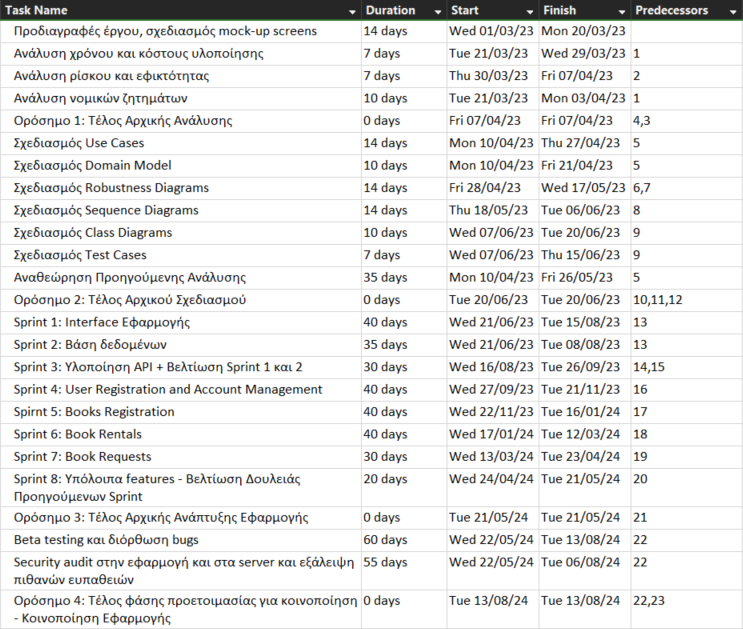
\includegraphics[width=\textwidth]{Project-Plan Table.png}}
	\caption{Πίνακας Χρονοπρογραμματισμού Project}
	\label{Πίνακας Χρονοπρογραμματισμού Project}
\end{figure}

Σημειώνω επίσης ότι έχουμε χωρίσει τα tasks μεταξύ των μελών της ομάδας, για το οποίο θα αναφερθούμε παραπάνω στην ενότητα \ref{Εντότητα Gantt Chart Έργου} (συγκεκριμένα στο Σχήμα \ref{Gantt chart χρονοπρογραμματισμού των tasks}.

Έχουμε επίσης κάνει εκτίμηση χρόνων χειρότερης περίπτωσης, καλύτερης περίπτωσης και έχουμε υπολογίσει τους χρόνους αναμενόμενης διάρκειας και τις διασπορές (Παραπάνω για αυτά στην ενότητα \ref{Ενότητα Pert Chart Έργου}, συγκεκριμένα στη Σχήμα \ref{Πίνακας Pert Data}.

\subsection{Gantt Chart Έργου}
\label{Εντότητα Gantt Chart Έργου}
Χρησιμοποιώντας τα δεδομένα στο Σχήμα \ref{Πίνακας Χρονοπρογραμματισμού Project} φτιάξαμε Gantt chart που απεικονίζει ποιες μέρες και για πόσο μεγάλο χρονικό διάστημα θα ασχοληθούμε (δηλαδή τουλάχιστον ένα μέλος της ομάδας θα ασχοληθεί) με το κάθε Task. To Gantt chart αυτό απαρτίζει το Σχήμα \ref{Gantt chart χρονοπρογραμματισμού των tasks}

\begin{figure}[H]
	\makebox[\textwidth]{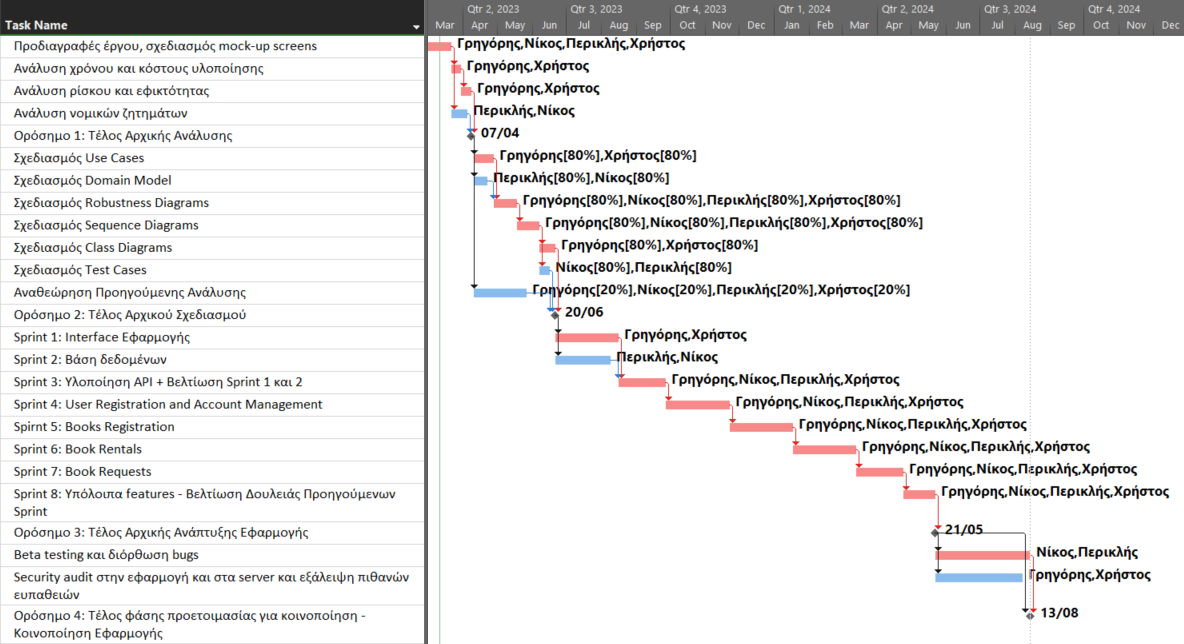
\includegraphics[width=\textwidth]{Project-Plan Gantt.png}}
	\caption{Gantt chart χρονοπρογραμματισμού των tasks}
	\label{Gantt chart χρονοπρογραμματισμού των tasks}
\end{figure}

Στην αριστερή στήλη φαίνονται τα ονόματα από τα task που αποσκοπούν σε κάθε bar του Gantt chart). Οπότε το κάθε όνομα είναι στην ίδια γραμμή με το bar που του αντιστοιχεί.

Σημειώνουμε ότι στο Gantt διάγραμμα παρουσιάζουμε επίσης ποια μέλη της ομάδας ορίσαμε υπεύθυνα για την διεκπεραίωση κάθε task. Οπότε δίπλα από κάθε κάθε bar παρουσιάζεται ένα ή παραπάνω ονόματα, μαζί με ένα ποσοστό για κάθε άτομο που δείχνει το ποσοστό του χρόνου του που θα αφοσιωθεί σε αυτό το task κατά τη διάρκεια διεκπεραίωσής του. Έχουμε θεωρήσει ότι αρκούν τα τέσσερα άτομα της ομάδας για τη διεκπεραίωση του έργου, οπότε χρησιμοποιήθηκαν τα ονόματά μας απευθείας, αντί για ονόματα ομάδων ή ρόλων για παράδειγμα.

Τέλος με κόκκινο χρώμα παραπάνω συμβολίζεται το κρίσιμο μονοπάτι για το Gantt chart. Αντίστοιχα με μπλέ χρώμα είναι τα μη κρίσιμα μονοπάτια. Σημειώνουμε εδώ ότι υπολογίζοντας τους χρόνους κανονικής εκτίμησης προέκυψε απευθείας ένα και μοναδικό κρίσιμο μονοπάτι, οπότε δεν χρειάστηκε να χρησιμοποιηθεί η διασπορά για την εκτίμηση για την εύρεση του κρίσιμου μονοπατιού, παρόλα αυτά έχουμε και πάλι συμπεριλάβει υπολογισμούς διασποράς και αναμενόμενης διάρκειας στο Σχήμα \ref{Πίνακας Pert Data}.

\subsection{Pert Chart Έργου}
\label{Ενότητα Pert Chart Έργου}

Χρησιμοποιώντας τα δεδομένα από το Σχήμα \ref{Πίνακας Χρονοπρογραμματισμού Project}, φτιάχνουμε Pert chart (Σχήμα \ref{Pert Chart Χρονοπρογραμματισμού Project}) που απεικονίζει τα task μαζί με τις εξαρτήσεις που προκύπτουν μεταξύ των tasks.

\textbf{Σημείωση:} Αποφασίσαμε να μην δείξουμε τις ημερομηνίες, τον χρόνο κανονικής εκτίμησης και τους χρόνους χειρότερης και καλύτερης περίπτωσης πάνω στο Pert chart επειδή το σχήμα θα γινόταν πολύ μεγάλο και δυσανάγνωστο. Για αυτό το λόγο δίνουμε τα στοιχεία που θα είχαμε κανονικά στο Pert chart στο συνοδευτικό Σχήμα \ref{Πίνακας Pert Data} ακριβώς από κάτω.

Εδώ πάλι με κόκκινο χρώμα συμβολίζεται το κρίσιμο μονοπάτι και με μπλέ συμβολίζονται τα μη κρίσιμα μονοπάτια.

\begin{figure}[H]
	\makebox[\textwidth]{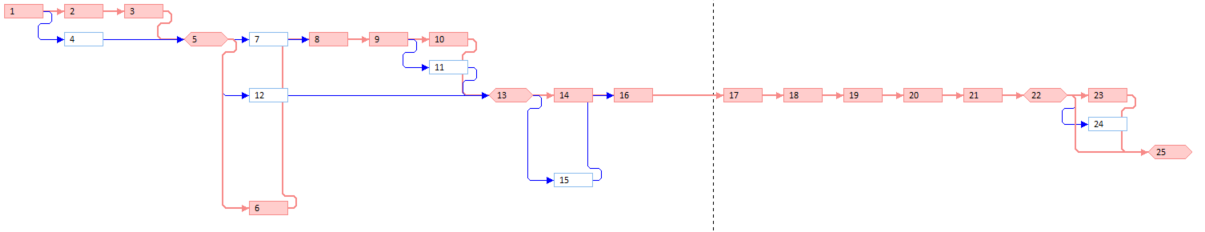
\includegraphics[width=\textwidth]{Project-Plan Pert.png}}
	\caption{Pert Chart Χρονοπρογραμματισμού Project}
	\label{Pert Chart Χρονοπρογραμματισμού Project}
\end{figure}

\begin{figure}[H]
	\makebox[\textwidth]{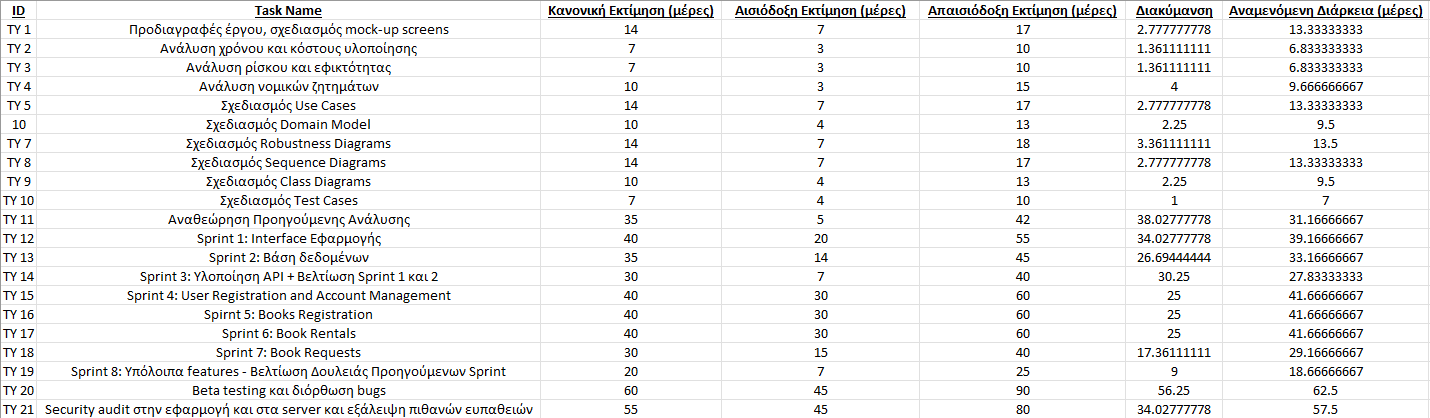
\includegraphics[width=\textwidth]{Project-Plan Pert Data.png}}
	\caption{Πίνακας Pert Data}
	\label{Πίνακας Pert Data}
\end{figure}

\section{Ανάλυση Κόστους Έργου}

\subsection{Άμεσα Κόστη}

Αρχικά θα υποθέσουμε ότι δεν χρειάστηκε να προσληφθούν παραπάνω άτομα, οπότε η ομάδα θα αποτελεί ται από τα 4 αρχικά μέλη.

Στα άμεσα κόστη θα συνυπολογίσουμε τα εξής:

\subsubsection{Μισθοί}
Εφόσον στον χρονοπρογραμματισμό παραπάνω δείχνουμε ότι κάθε άτομο δουλεύει μόνιμα και δεν υπάρχουν κενά, δεν χρειάζεται να αναλύσουμε το κόστος ανά task, ειδικά επειδή πολλές φορές μέλη της ομάδας κάνουν πολλά task ταυτόχρονα.

Οπότε θα ορίσουμε ότι κάθε άτομο δουλεύει 8 ώρες την ημέρα, 5 ημέρες την εβδομάδα, με συνολικό αριθμό ημερών εργασίας να είναι ίσο με 532 (1 Μαρτίου 2023 - 13 Αυγούστου 2024 με αφαιρεμένες τα σαββατοκύριακα και τις αργίες). Επίσης θα θεωρήσουμε ωριαίο μισθό 35\euro\space ανά ώρα (μαζί με ασφάλιση). Άρα το συνολικό κόστος εργασίας για τα 4 άτομα θα είναι:

$μισθοι = μερες \cdot \frac{ωρες}{μερα} \cdot \frac{ευρω}{ωρα} \cdot ατομα = 532 * 8 * 35 * 4 = 595840\euro$

\subsubsection{Υπόλοιπα Κόστη}

Στα υπόλοιπα κόστη θα συνυπολογίσουμε κόστος για servers, διαφημίσεις, security audit από έμπιστη εταιρεία και κόστος σύμβουλων νομικών ειδικών. Αυτά τα κόστη φαίνονται παρακάτω:

\begin{itemize}
	\item \textbf{Servers:} 1400\euro

		Υποθέτουμε ότι μέχρι την δημοσίευση της εφαρμογής έχουμε νοικιάσει servers για συνολικά 14 μήνες (από τέλη Ιουνίου 2023 μέχρι αρχές Αυγούστου 2024), οπότε θεωρώντας κόστος 100\euro\space ανά μήνα το συνολικό κόστος είναι 1400\euro.

	\item \textbf{Διαφημίσεις:} 6000\euro

		Υποθέτουμε ότι μέχρι την δημοσίευση της εφαρμογής έχουμε διαφημίσει για συνολικά τρεις μήνες. Θεωρούμε ότι διαφημίζουμε μέσω social media και το συνολικό κόστος είναι 2000\euro\space ανά μήνα το συνολικό κόστος είναι 6000\euro.

	\item \textbf{Security audit:} 1500\euro

		Αναζητώντας για τιμές στο διαδίκτυο βλέπουμε ένα security audit μπορεί να κοστίσει από 700 - 2500\textdollar\space (\href{https://www.getastra.com/blog/security-audit/it-security-audit-cost/}{Πηγή}), οπότε υπολογίζουμε γύρω στα 1500\euro.

	\item \textbf{Νομική Συμβουλή:} 1500\euro

		Υποθέτουμε ότι για τη συνολική βοήθεια που χρειαζόμαστε αποσκοπεί σε 10 - 15 ώρες συμβουλών, με ανταμοιβή 70 - 100\euro\space περίπου ανά ώρα, οπότε θεωρήσαμε 1500\euro\space περίπου.
\end{itemize}

\subsection{Έμμεσο Κόστος}

Θεωρούμε ότι νοικιάζουμε γραφείο για την ομάδα από όπου θα εκπονούμε τη δουλειά. Οπότε για έμμεσα κόστος θα έχουμε το νοίκι, το ρεύμα, το νερό, τα κοινόχρηστα και τη βενζίνη για μετακίνηση στο γραφείο. Τα κόστη αυτά αναλύονται παρακάτω:

\begin{itemize}
	\item \textbf{Νοίκι:} 10800\euro

		Υποθέτουμε ότι το νοίκι είναι 600\euro\space ανά μήνα και ότι το νοικιάζουμε για 18 μήνες μέχρι την δημοσίευση του έργου. Άρα συνολικά 10800\euro.

	\item \textbf{Ρεύμα:} 1800\euro

		Υποθέτουμε ότι το ρεύμα είναι 100\euro\space ανά μήνα και ότι το νοικιάζουμε για 18 μήνες μέχρι την δημοσίευση του έργου. Άρα συνολικά 1800\euro.

	\item \textbf{Νερό:} 720\euro

		Υποθέτουμε ότι το νερό είναι 40\euro\space ανά μήνα και ότι το νοικιάζουμε για 18 μήνες μέχρι την δημοσίευση του έργου. Άρα συνολικά 720\euro.

	\item \textbf{Κοινόχρηστα:} 900\euro

		Υποθέτουμε ότι τα κοινόχρηστα είναι 50\euro\space ανά μήνα και ότι το νοικιάζουμε για 18 μήνες μέχρι την δημοσίευση του έργου. Άρα συνολικά 900\euro.
\end{itemize}

\subsection{Συνολική εκτίμηση κόστους}

Από τα άμεσα κόστη του κεφαλαίο 3.1 και τα έμμεσα κόστη του κεφαλαίου 3.2 έχουμε το εξής συνολικό κόστος:

$Συνολο = 595840 + 1400 + 6000 + 1500 + 1500 + 10800 + 1800 + 720 + 900 \approx 620500\euro$

\section{Συμμετοχή και Ρόλοι στη Συγγραφή του Κειμένου}
\begin{enumerate}
	\item \textbf{Γρηγόρης Καπαδούκας:} Author
	\item \textbf{Χρήστος Μπεστητζάνος:} Editor, Contributor
	\item \textbf{Νικόλαος Αυγέρης:} Peer Reviewer
\end{enumerate}
\end{document}
